\subsubsection{Dịch vụ thanh toán (payment service)}

% Mục đích:
Dịch vụ thanh toán (payment service) chịu trách nhiệm quản lý thông tin các gói dịch vụ (\texttt{plans}), quản lý thuê bao người dùng (\texttt{subscriptions}) của người dùng và tích hợp các cổng thanh toán.
Sơ đồ tổng quan về dịch vụ thanh toán:

\begin{figure}[H]
\centering
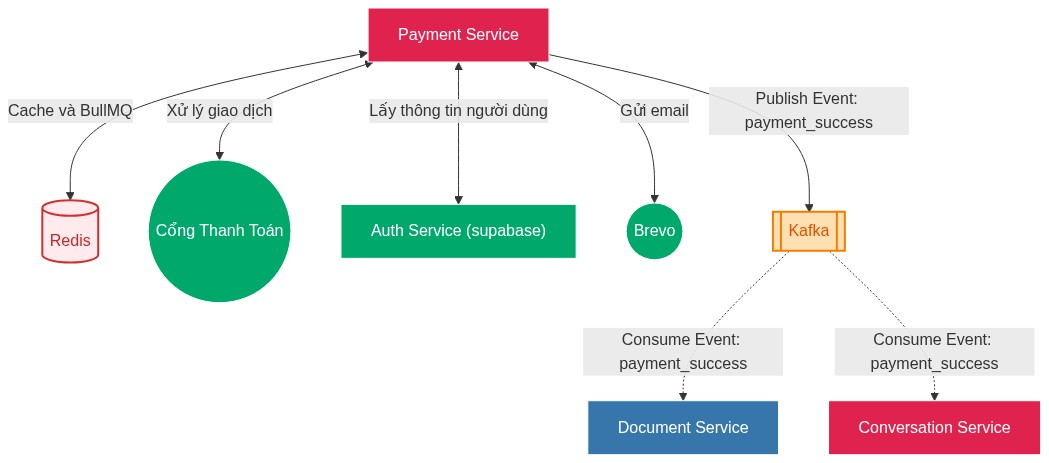
\includegraphics[width=0.95\textwidth]{pictures/payment-kafka-event.png}
\caption{Sơ đồ tổng quan dịch vụ thanh toán}
\end{figure}

\paragraph{Quản lý Gói dịch vụ (Plans)}

Cho phép hệ thống
định nghĩa và cung cấp
các gói dịch vụ khác nhau tới người dùng.

\begin{itemize}
\item \textbf{Tạo mới gói dịch vụ}:
Cho phép quản trị viên (ADMIN)
thiết lập cấu hình gói dịch vụ mới
bao gồm các thông số:
tên gói (ví dụ: VIP 1 tháng),
thời hạn sử dụng,
giá tiền,
trạng thái hoạt động
và mô tả các tính năng đi kèm
(ví dụ: Quyền sử dụng mô hình suy luận AI, Voice, xử lý tài liệu nâng cao).

\item \textbf{Truy xuất danh sách gói}:
Lấy danh sách toàn bộ
các gói dịch vụ hiện có
trên hệ thống.
% để hiển thị cho người dùng.
Chức năng này được phân trang thông qua hai tham số \texttt{skip} và \texttt{limit}.

\item \textbf{Cơ chế Cache với Redis}:
Lưu thông tin cache danh sách các plan vào Redis.
Khi người dùng yêu cầu xem danh sách gói đăng ký, hệ thống sẽ ưu tiên đọc từ Redis.
Nếu cache trống, hệ thống sẽ truy xuất CSDL, trả về kết quả cho client
và lưu lại kết quả đó vào Redis cho các yêu cầu sau.

\item \textbf{Lưu trữ gói thuê bao VIP}:
Cho phép quản trị viên tạm dừng
% cung cấp
các gói dịch vụ cũ.

\end{itemize}

% Các API chính trong tài liệu Swagger API của Dịch vụ thanh toán (payment service):

\begin{figure}[H]
\centering
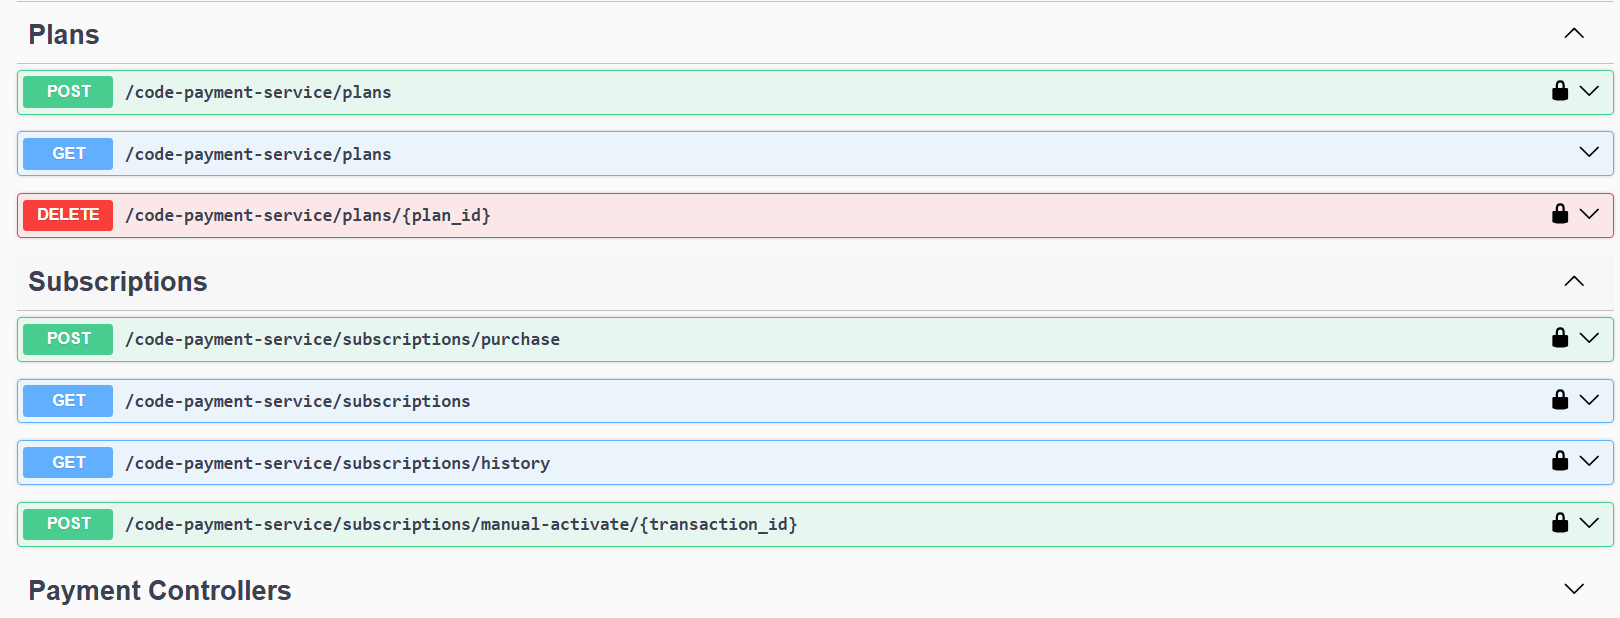
\includegraphics[width=0.9\textwidth]{pictures/payment-swagger.png}
\caption{Tài liệu Swagger API dịch vụ thanh toán}
\end{figure}

\paragraph{Quản lý Thuê bao (Subscriptions) và Giao dịch}

Quản lý thông tin
đăng ký dịch vụ của người dùng
và các giao dịch phát sinh:

\begin{itemize}
\item \textbf{Mua gói}:
Người dùng khởi tạo yêu cầu thanh toán cho một gói dịch vụ cụ thể. Hệ thống tiếp nhận mã gói (\texttt{plan\_id}) và đường dẫn chuyển hướng (\texttt{redirect\_url}) để tạo link thanh toán và đưa người dùng tới cổng thanh toán.
Tích hợp chức năng tự động hủy giao dịch nếu hết thời gian chờ thanh toán (timeout) cấu hình trong Redis.
Gửi sự kiện thanh toán thành công lên Kafka.
Gửi email thông báo xác nhận thanh toán thành công cho người dùng.

\item \textbf{Tra cứu thông tin thuê bao}:
Cho phép người dùng xem thông tin chi tiết
à thời hạn của gói dịch vụ hiện tại mà họ đang sở hữu.

\item \textbf{Tra cứu lịch sử giao dịch}:
Cung cấp danh sách lịch sử các giao dịch thanh toán trước đó của người dùng, hỗ trợ phân trang để dễ dàng theo dõi.

\item \textbf{Kích hoạt giao dịch thủ công}:
Tính năng dành cho ADMIN để can thiệp kích hoạt thủ công một giao dịch (\texttt{transaction\_id}) thành công, dùng trong các trường hợp xử lý sự cố.

\end{itemize}

\paragraph{Tích hợp Cổng thanh toán}

\begin{itemize}
\item \textbf{Xử lý Callback (IPN)}:
Cung cấp các endpoint (nhận cả phương thức \texttt{GET} và \texttt{POST}) để cổng thanh toán có thể âm thầm gọi về hệ thống (giao tiếp server-to-server) nhằm cập nhật trạng thái giao dịch một cách chính xác và bảo mật nhất.

\item \textbf{Xử lý Return URL}:
Cung cấp các endpoint (nhận cả \texttt{GET} và \texttt{POST}) để tiếp nhận và điều hướng giao diện người dùng ngay sau khi họ hoàn tất thao tác thanh toán trên trang của đối tác.

\end{itemize}

Trong quá trình phát triển dự án, do các dịch vụ thanh toán sẵn có chưa hỗ trợ tốt các cổng thanh toán phổ biến tại Việt Nam (như VNPay, ZaloPay, MoMo, SePay, ...), dịch vụ thanh toán này đã được tự thiết kế, phát triển và triển khai độc lập trên nền tảng Heroku.

Quy trình đóng gói và vận hành:
\begin{itemize}
\item Dịch vụ được đóng gói tự động bằng Docker do Heroku xử lý.
\item Tự động chạy và triển khai lên Heroku khi vượt qua các bước kiểm thử (tests) trong CI/CD của GitHub Actions.
\item Kết nối trực tiếp với CSDL Postgres (Neon), Kafka và Redis để vận hành hàng đợi BullMQ.
\end{itemize}

Triển khai Dịch vụ thanh toán (payment service) độc lập trên Heroku:

\begin{figure}[H]
\centering
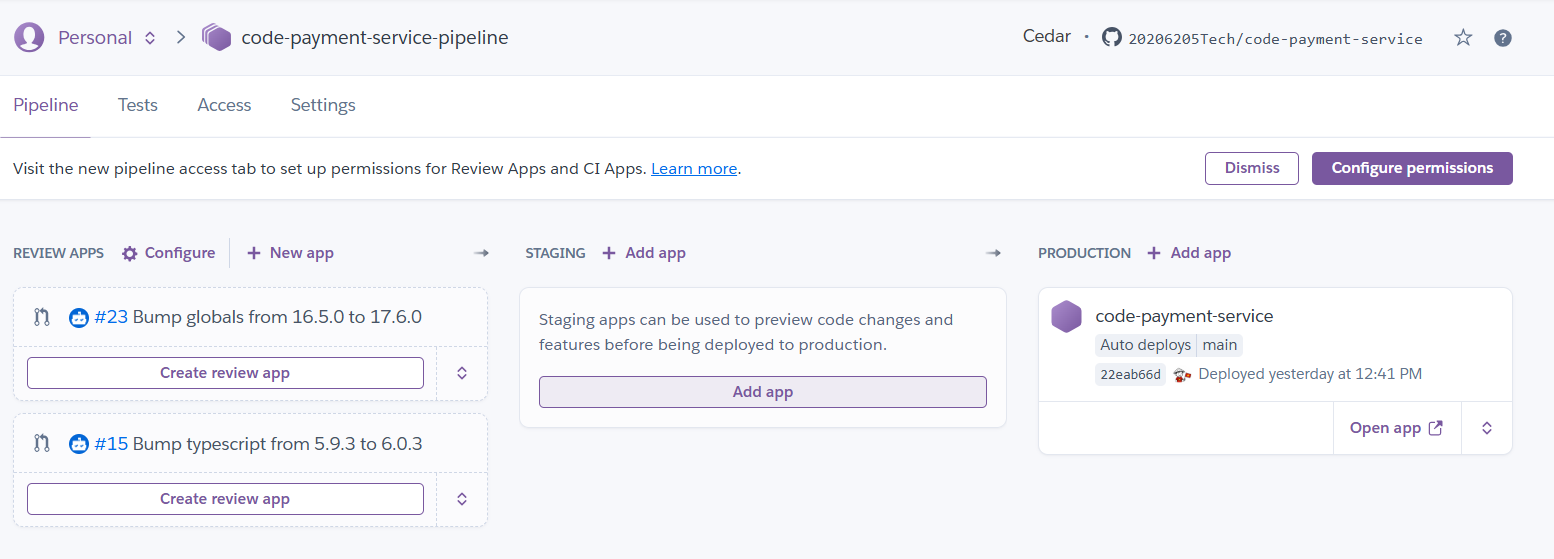
\includegraphics[width=0.95\textwidth]{pictures/payment-heroku.png}
\caption{Kết quả triển khai dịch vụ thanh toán trên Heroku}
\end{figure}

Các bước CI/CD tự động chạy kiểm thử trên GitHub Actions:
Dịch vụ sử dụng \textbf{Testcontainers} (cho Postgres, Redis và Kafka) để tự động khởi chạy các container Docker độc lập ngay trong quá trình chạy kiểm thử tích hợp, đảm bảo tính đúng đắn của mã nguồn trước khi triển khai.
Hàng đợi tác vụ bất đồng bộ \textbf{BullMQ} (vận hành trên Redis) được tích hợp để quản lý và tự động xử lý hủy các giao dịch thanh toán quá hạn nếu hết thời gian chờ.

Dữ liệu gói thuê bao VIP được cache trong Redis:

\begin{figure}[H]
\centering
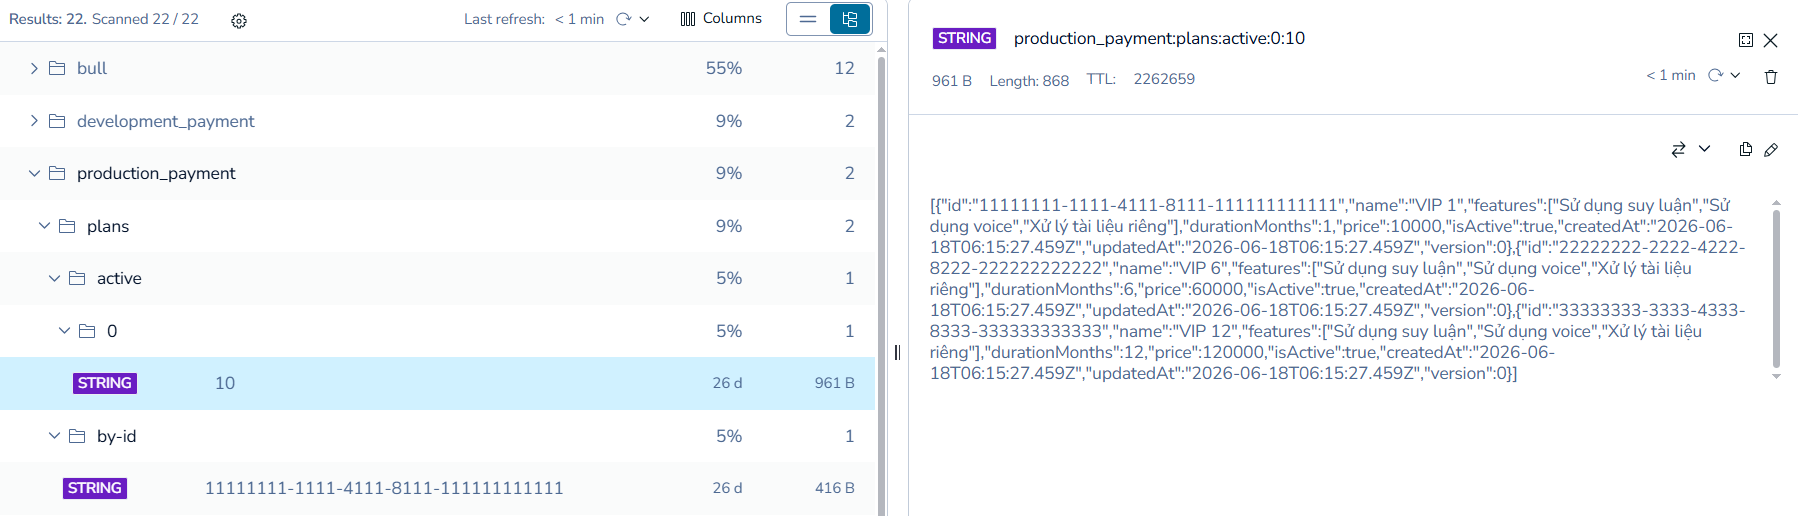
\includegraphics[width=0.95\textwidth]{pictures/payment-redis-v2.png}
\caption{Dữ liệu gói thuê bao VIP được cache trong Redis}
\end{figure}

Thông tin kiểm tra tự động của Pull Request của payment service trên GitHub:

\begin{figure}[H]
\centering
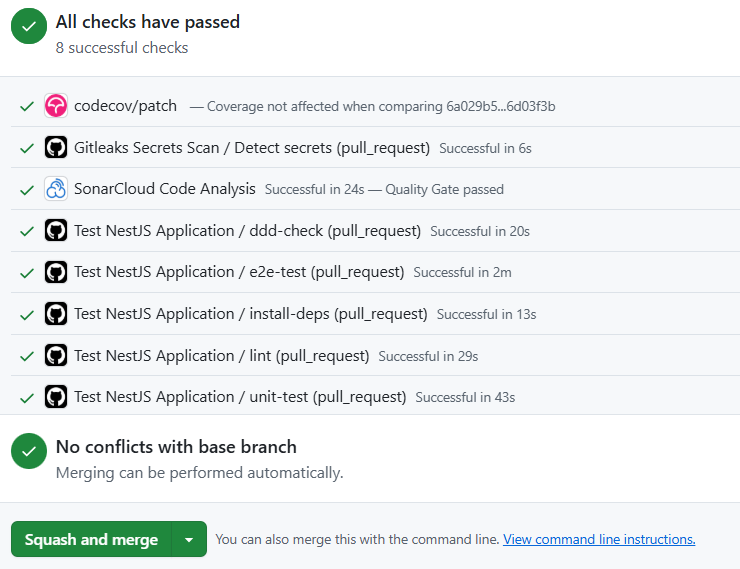
\includegraphics[width=0.8\textwidth]{pictures/payment-PR.png}
\caption{Kiểm tra Pull Request của payment service trên GitHub}
\end{figure}

\begin{figure}[H]
\centering
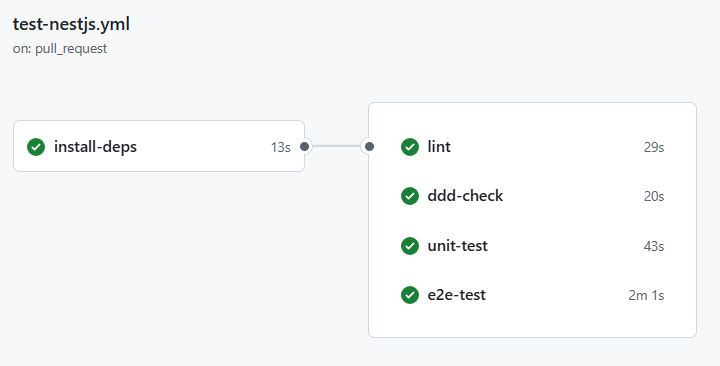
\includegraphics[width=0.95\textwidth]{pictures/payment-test.png}
\caption{Quy trình chạy Test của payment service trên GitHub Actions}
\end{figure}

Quản lý di chuyển CSDL tự động trong GitHub Actions:

\begin{figure}[H]
\centering
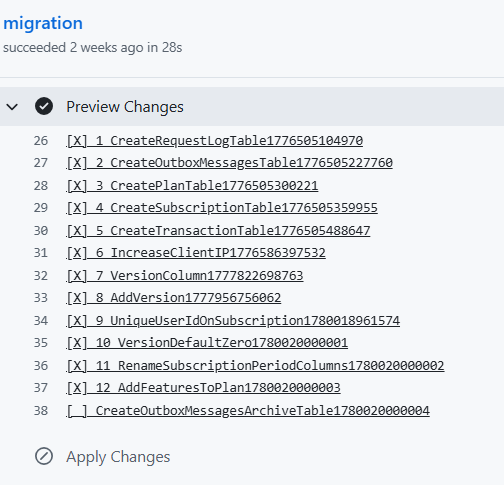
\includegraphics[width=0.8\textwidth]{pictures/payment-database-migration.png}
\caption{Quản lý di chuyển CSDL trên GitHub Actions}
\end{figure}

Các bảng trong CSDL của dịch vụ thanh toán (payment service):

\begin{figure}[H]
\centering
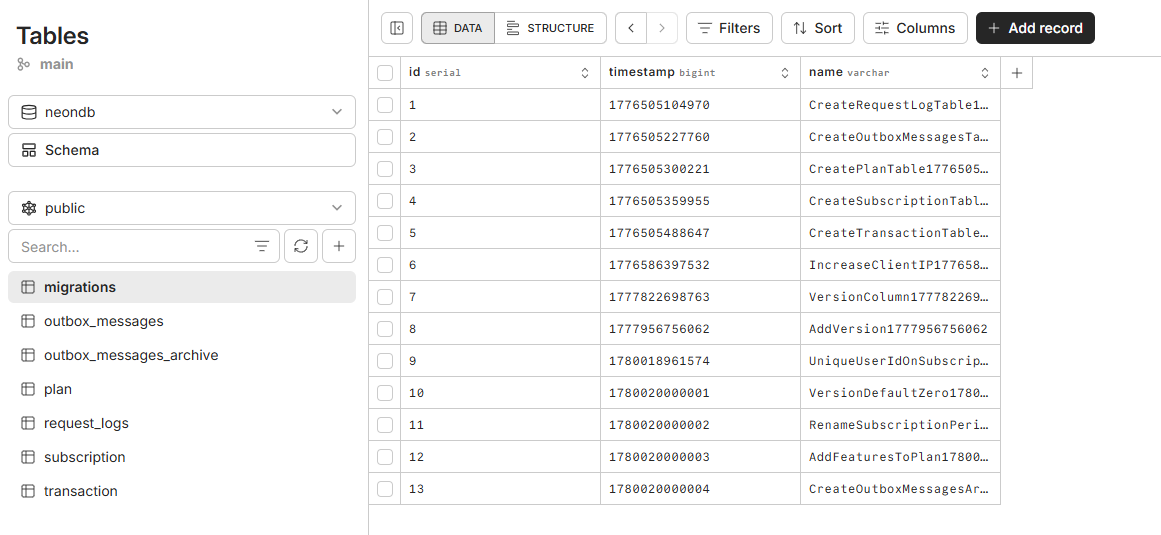
\includegraphics[width=0.95\textwidth]{pictures/payment-database.png}
\caption{Cấu hình các bảng CSDL của dịch vụ thanh toán}
\end{figure}

\paragraph{Sự kiện Thanh toán thành công (Subscription Purchased Event)}

Khi giao dịch thanh toán gói dịch vụ thành công,
Dịch vụ thanh toán sẽ tạo và phát hành (publish) sự kiện lên
Kafka để đồng bộ quyền hạn người dùng.

\subparagraph{Chi tiết sự kiện}
\begin{itemize}
\item \textbf{Tên Sự kiện}: \texttt{SubscriptionPurchasedEvent}
\item \textbf{Topic}: \texttt{dev-payment-events} hoặc \texttt{prod-payment-events}
\item \textbf{Mã hóa (Compression)}: \texttt{GZIP}
\item \textbf{Phân vùng khóa (Message Key)}: \texttt{userId} (đảm bảo tính tuần tự của các sự kiện liên quan đến cùng một người dùng trên cùng một partition).
\end{itemize}

\subparagraph{Cấu trúc dữ liệu sự kiện}
Dữ liệu sự kiện được gửi dưới dạng chuỗi JSON có cấu trúc như sau:

\begin{table}[H]
\centering
\begin{tabular}{|l|l|l|}
\hline
\textbf{Thuộc tính} & \textbf{Kiểu dữ liệu} & \textbf{Mô tả} \\ \hline
\texttt{subscriptionId} & String (UUID) & Mã định danh duy nhất của thuê bao \\ \hline
\texttt{userId} & String (UUID) & Mã định danh người dùng mua gói \\ \hline
\texttt{planId} & String (UUID) & Mã định danh gói dịch vụ đã mua \\ \hline
\texttt{periodStart} & String & Thời điểm bắt đầu hiệu lực gói dịch vụ \\ \hline
\texttt{periodEnd} & String & Thời điểm kết thúc hiệu lực gói dịch vụ \\ \hline
\texttt{version} & Number & Số phiên bản của sự kiện (dùng để quản lý xung đột) \\ \hline
\texttt{occurredAt} & String & Thời điểm sự kiện phát sinh thực tế trên máy chủ \\ \hline
\end{tabular}
\caption{Cấu trúc dữ liệu sự kiện SubscriptionPurchasedEvent}
\end{table}

\begin{figure}[H]
\centering
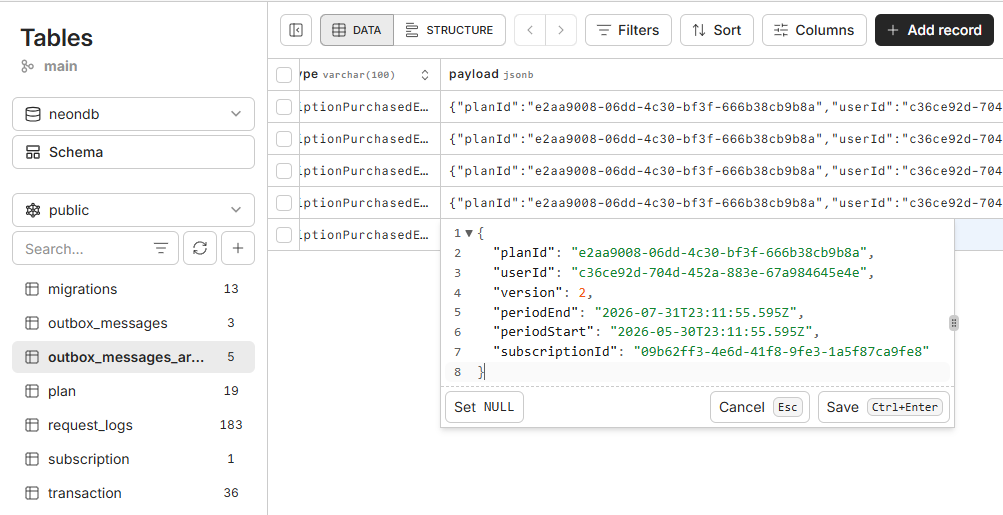
\includegraphics[width=0.7\textwidth]{pictures/event-outbox.png}
\caption{Thông tin sự kiện được lưu trong bảng Outbox}
\end{figure}

\subparagraph{Cách các dịch vụ khác tiếp nhận và xử lý sự kiện}
Sự kiện này được tiêu thụ (consume) song song bởi hai dịch vụ: \textbf{dịch vụ văn bản (document service - Python)} (Consumer Group: \texttt{document-service-group}) và \textbf{dịch vụ trò chuyện (conversation service - NestJS)} (Consumer Group: \texttt{conversation-service-group}) để đồng bộ quyền lợi gói VIP của người dùng theo các bước tuần tự sau:

\begin{enumerate}
\item \textbf{Lắng nghe và giải mã}: Consumer lắng nghe sự kiện từ topic tương ứng, phân tích và giải mã JSON payload nhận được.
\item \textbf{Khởi tạo giao dịch và khóa dòng}: Khởi tạo một giao dịch CSDL (\textbf{Database Transaction}) để thực hiện cập nhật bảng thông tin thuê bao của người dùng. Để tránh tranh chấp dữ liệu (Race Condition) khi có nhiều sự kiện xử lý song song, hệ thống kích hoạt khóa ghi bi quan (\textbf{Pessimistic Write Lock} hoặc cơ chế tương đương) trên dòng dữ liệu của \texttt{userId} đó.
\item \textbf{So sánh phiên bản lớn hơn}: So sánh trường \texttt{version} của sự kiện nhận được với \texttt{version} hiện tại trong CSDL.
Nếu phiên bản của sự kiện lớn hơn,
tiến hành cập nhật thông tin thuê bao
(\texttt{period\_start}, \texttt{period\_end}, \texttt{subscription\_id}, \texttt{version})
và đặt trạng thái kích hoạt
VIP (\texttt{is\_active = True}).
\item \textbf{Xử lý phiên bản nhỏ hơn hoặc bằng}: Nếu phiên bản nhận được nhỏ hơn hoặc bằng, hệ thống sẽ bỏ qua (SKIP) sự kiện vì đã tồn tại bản cập nhật mới hơn trong CSDL (cơ chế Version Control giúp ngăn chặn lỗi out-of-order event).
\item \textbf{Kích hoạt quyền VIP}: Sau khi cập nhật CSDL thành công, hệ thống mở khóa người dùng và kích hoạt các quyền lợi VIP tương ứng (như trò chuyện thoại nâng cao, mô hình suy luận, xử lý tài liệu).
\end{enumerate}

\paragraph{Cơ chế Instant Payment Notification (IPN)}

% IPN (Instant Payment Notification)
được sử dụng để
Đơn vị cung cấp dịch vụ thanh toán - Payment Service Provider (PSP)
thông báo kết quả giao dịch một cách không đồng bộ cho
Đơn vị sử dụng dịch vụ - Payment Service Consumer (PSC).

\begin{figure}[H]
\centering
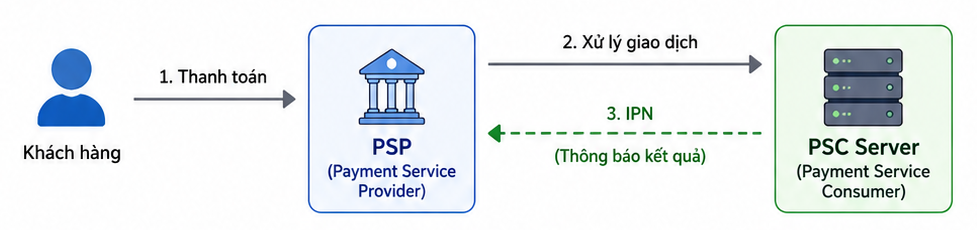
\includegraphics[width=0.9\textwidth]{pictures/payment-ipn-i1.png}
\caption{Sơ đồ nguyên lý hoạt động của IPN}
\end{figure}

Sau khi khách hàng hoàn tất thanh toán, kết nối mạng của họ có thể bị gián đoạn hoặc họ có thể tắt trình duyệt trước khi được chuyển hướng về trang Web của hệ thống (Return URL). Cơ chế IPN đảm bảo rằng máy chủ của hệ thống vẫn nhận được kết quả cuối cùng một cách độc lập từ đối tác để cập nhật trạng thái đơn hàng một cách chính xác.

\begin{figure}[H]
\centering
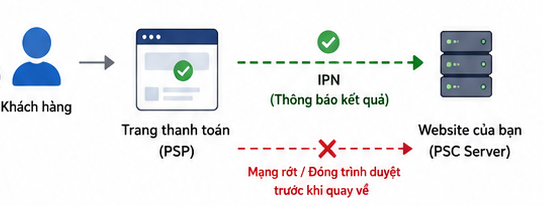
\includegraphics[width=0.9\textwidth]{pictures/payment-ipn-i2.png}
\caption{Mô phỏng luồng cập nhật trạng thái qua IPN}
\end{figure}

\paragraph{Thiết kế hệ thống theo Domain-Driven Design (DDD)}

Dự án được thiết kế theo mô hình phát triển hướng tên miền (Domain-Driven Design - DDD) kết hợp với kiến trúc lục giác (Hexagonal Architecture).
Để demo khả năng thay đổi linh
hoạt các dịch vụ tích hợp bên ngoài,
hệ thống cho phép cấu hình cổng thanh toán
mặc định thông qua biến
môi trường \texttt{PAYMENT\_DEFAULT\_PROVIDER}.
Nhờ áp dụng Dependency Inversion thông
qua các Interface,
việc chuyển đổi hoặc bổ
sung các cổng thanh toán mới
được thực hiện vô cùng dễ dàng
mà không làm ảnh
hưởng đến nghiệp vụ cốt lõi.

% Giao diện demo thanh toán qua VNPay:

\begin{figure}[H]
\centering
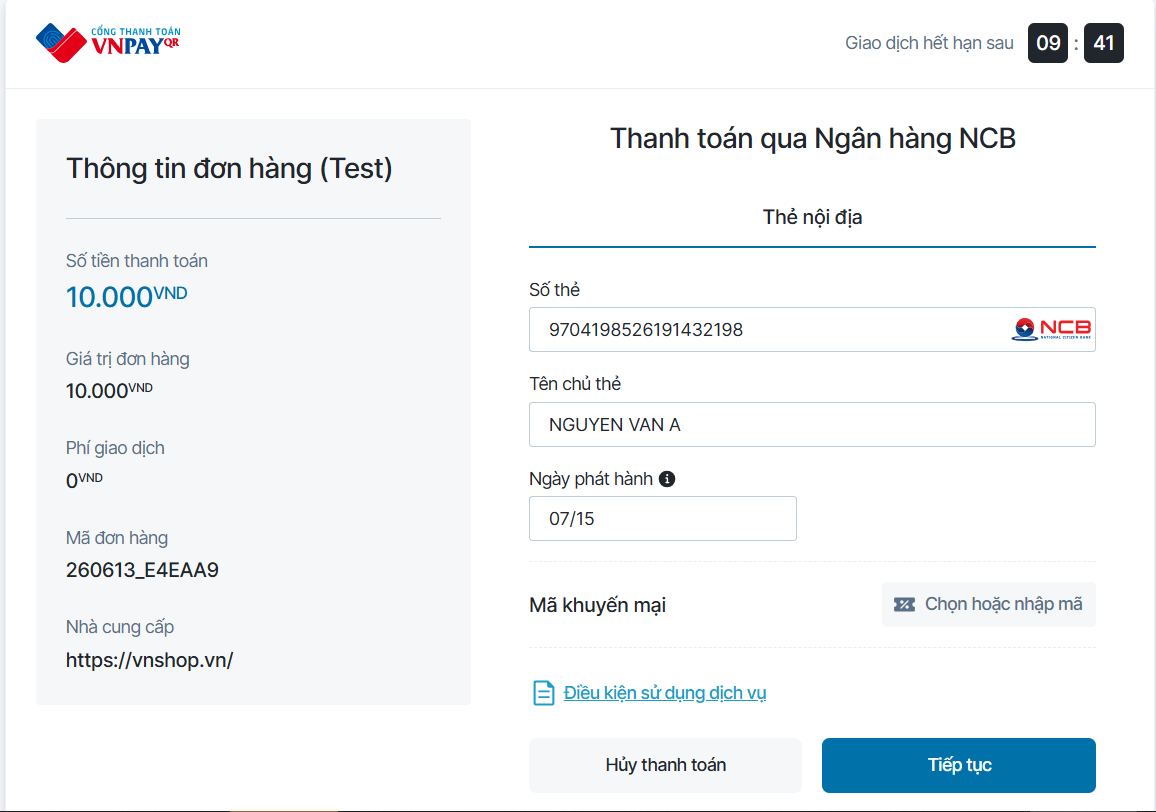
\includegraphics[width=0.64\textwidth]{pictures/payment-vnpay.png}
\caption{Giao diện thanh toán VNPay}
\end{figure}

\newpage
Giao diện demo thanh toán qua MoMo:

\begin{figure}[H]
\centering
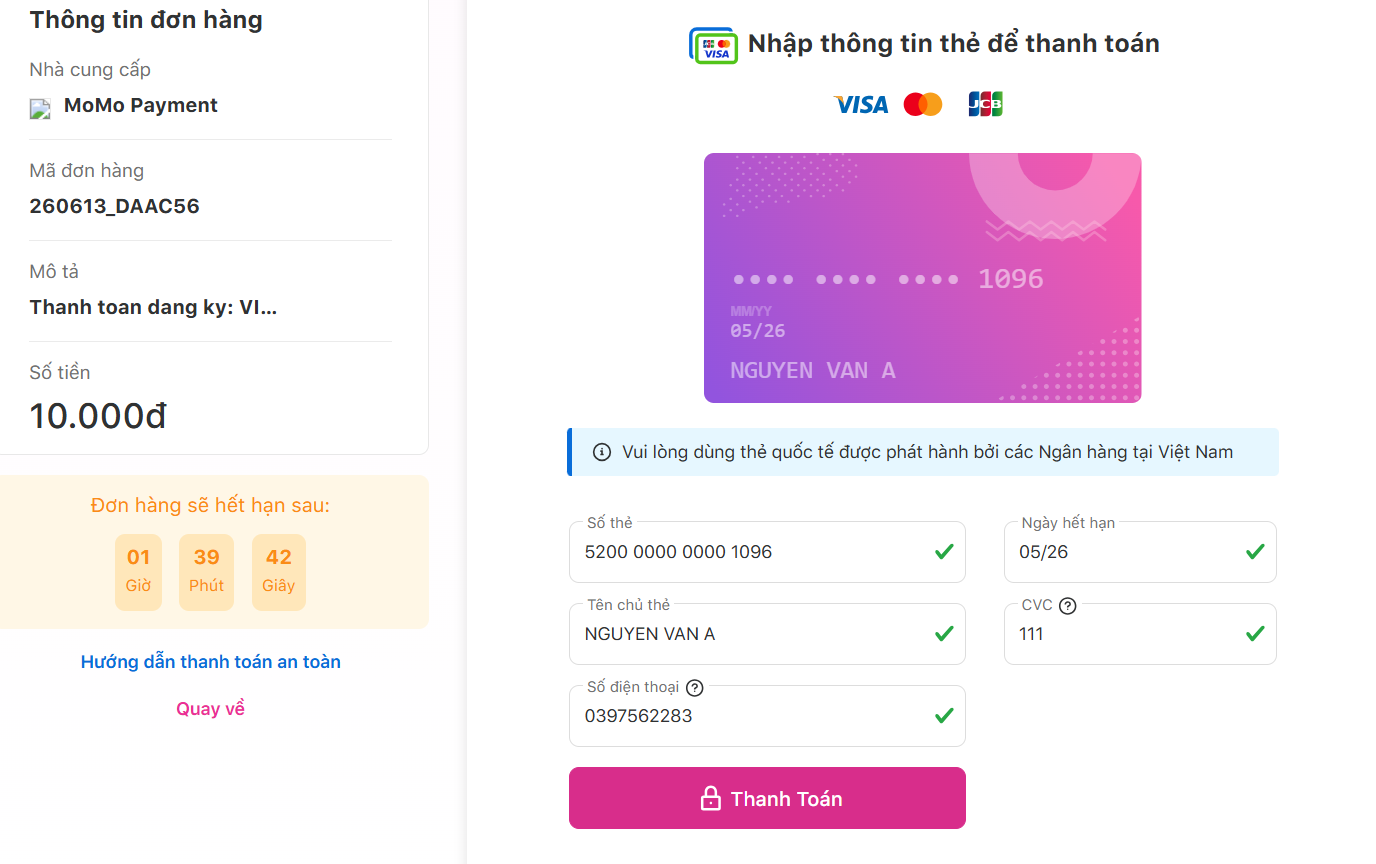
\includegraphics[width=0.99\textwidth]{pictures/payment-momo.png}
\caption{Giao diện thanh toán MoMo}
\end{figure}

Giao diện demo thanh toán qua ZaloPay:

\begin{figure}[H]
\centering
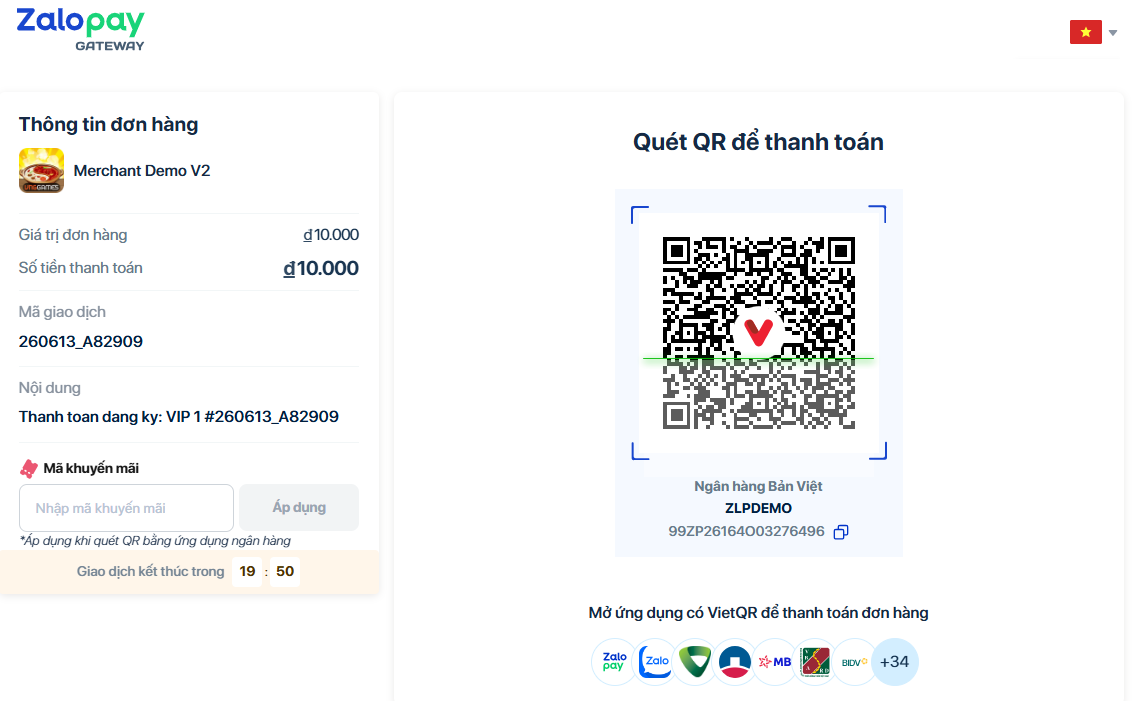
\includegraphics[width=0.99\textwidth]{pictures/payment-zalo.png}
\caption{Giao diện thanh toán ZaloPay}
\end{figure}

\newpage

Giao diện demo thanh toán qua SePay:

\begin{figure}[H]
\centering
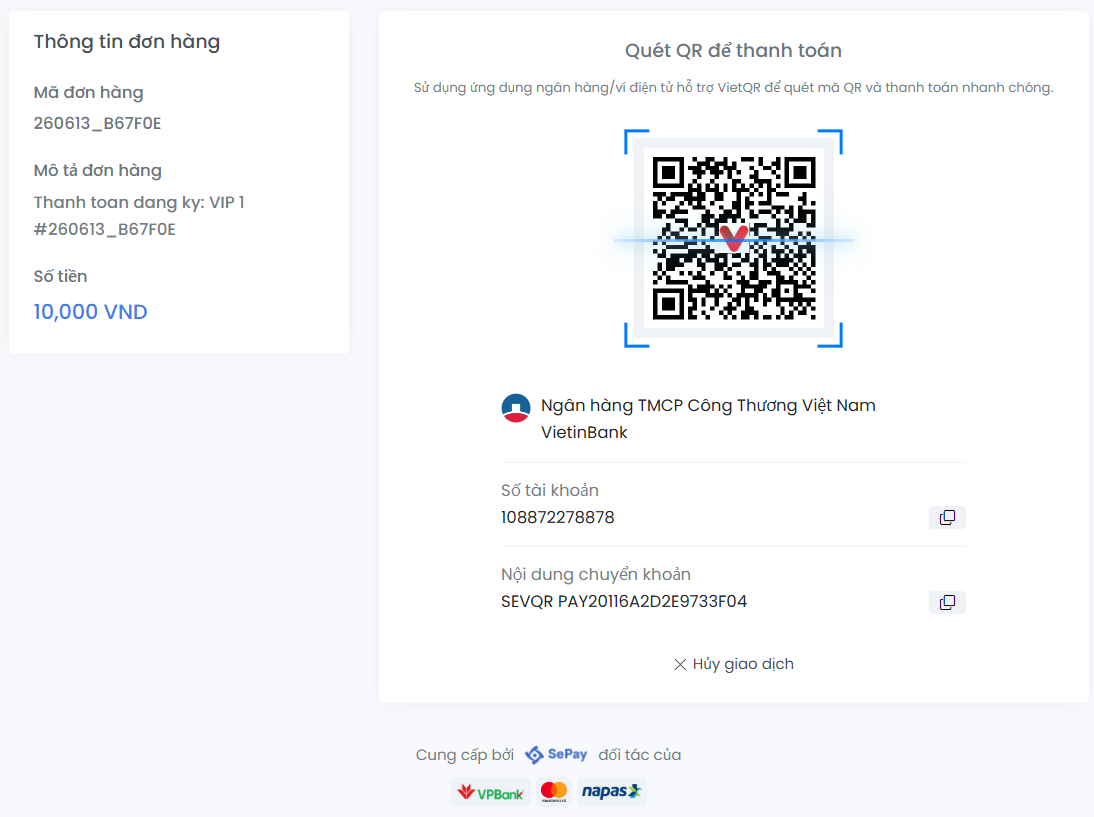
\includegraphics[width=0.95\textwidth]{pictures/payment-sepay.png}
\caption{Giao diện thanh toán SePay}
\end{figure}

Mẫu email gửi cho người dùng khi thanh toán thành công:

\begin{figure}[H]
\centering
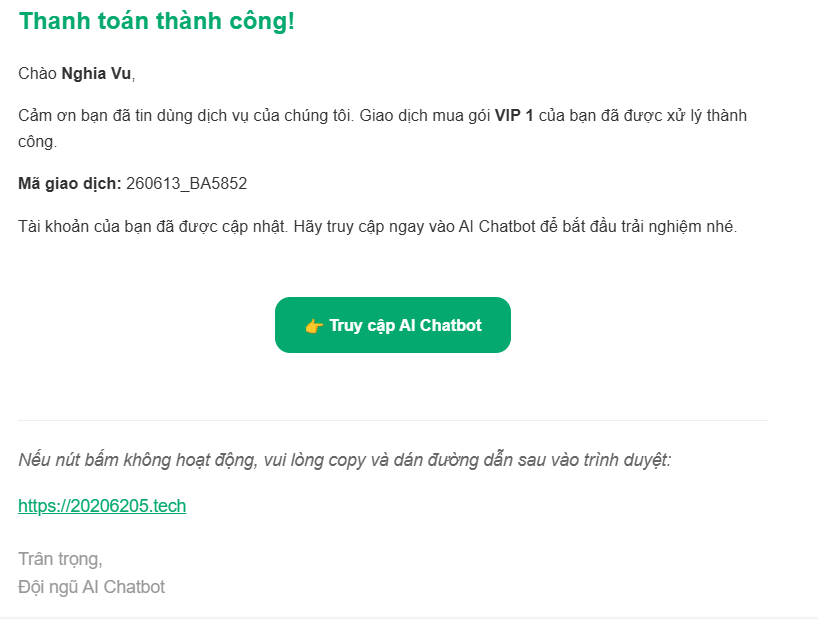
\includegraphics[width=0.95\textwidth]{pictures/payment-mail.png}
\caption{Email thông báo thanh toán thành công}
\end{figure}
\newpage
